\documentclass{article}

\usepackage{geometry}
\usepackage{amsfonts, amsmath, amssymb, amsthm}
\usepackage{enumitem}
\usepackage{commands}
\usepackage{mathtools}
\usepackage{hyperref}
\hypersetup{colorlinks, linkcolor={blue}, citecolor={blue}, urlcolor={blue}}

\usepackage{tikz-cd}
\newcommand{\Card}{\operatorname{Card}}

\begin{document}
\puttitle{Covering spaces over the wrong space}\self

For the general theory of covering spaces to work, we usually impose the following conditions on the base space $X$:
\begin{enumerate}[label=(\roman*)]
    \item\label{con} $X$ is connected;
    \item\label{lpc} $X$ is locally path connected;
    \item\label{semi} $X$ is semilocally simply connected.
\end{enumerate}

Recall that \ref{semi} means that there is a neighborhood $U$ of any $x\in X$, such that the homomorphism $\pi_1(U,x)\longrightarrow\pi_1(X,x)$ induced by inclusion is trivial. Equivalently, this requires that every loop in $U$ be null-homotopic in $X$. So the basepoint is not important here.

Given these conditions, it is well known how to establish the existence of universal covers and the Galois correspondence. But in this note, we are interested in the following result.

\begin{theorem}\label{thm}
    Suppose that the base space $X$ satisfies \ref{lpc} and \ref{semi}. Let $q:Z\longrightarrow Y$ and $p:Y\longrightarrow X$ be coverings. The the composite $Z\longrightarrow X$ is also a covering.
\end{theorem}

\begin{proof}
    Fix $x_0\in X$ and let $U$ be the neighborhood guaranteed by \ref{semi}. By shrinking $U$, we may assume that it is open and path connected. I claim that $U$ is a fundamental neighborhood, i.e., the covering $p$ restricts to a trivial cover over $U$.
    
    By path lifting, any (path) connected component $V$ of $p^{-1}(U)$ maps onto $U$ via the local homeomorphism. Thus it suffices to check that $\left.p\right\vert_{V}$ is injective. Suppose that $x,y\in V$ and $p(x)=p(y)$. Any path in $V$ connecting $x$ to $y$ descends to a loop based at $p(x)$, which can be shrunk into $p(x)$ by assumption. The square of this homotopy has three of its edges being the constant path at $p(x)$. Hence $x=y$ by uniqueness of homotopy lifting.

    Now, notice that the same applies to $V$ and the covering $q$. $V$ is open and path connected by definition, and by homotopy lifting, any loop in $V$ is clearly null-homotopic in $Y$. Hence $q^{-1}(V)$ is a disjoint union of copies of $V\simeq U$, and $(p\circ q)^{-1}(U)$ is a disjoint union of these sets. This completes the proof.
\end{proof}

\begin{remark}
    The proof also shows that any cover of a simply connected space is trivial.
\end{remark}

In this note I try to understand how this theorem depends on the conditions.

\section{Example 1}

Let's first consider $X=\Q$ with the standard topology. Note that it does satisfy \ref{semi}, but is obviously not locally path connected or locally simply connected.

\begin{theorem}
    We have a bijection
    \[\begin{tikzcd}[row sep=small]
        \left\{ \text{covering }p:Y\longrightarrow\Q \right\} \arrow[r, yshift=0.5ex, "1:1"] & \left\{ \text{continuous }v:\Q\longrightarrow\Card \right\} \arrow[l, yshift=-0.5ex]
    \end{tikzcd}\]
    given by sending $p$ to the map assigning to each rational number $x$ the size of the fiber $p^{-1}(x)$. Here $\Card$ is the discrete class (or a big set) of nonzero cardinals.
\end{theorem}

\begin{proof}
    As true for any covering, the size of fiber function is locally constant. Hence this map $p\mapsto v$ is well-defined. It is obviously surjective. To show injectivity, it remains to prove that any covering $q$ of constant fiber size $\kappa$ over an open subset $U\subset\Q$ is trivial. 

    Clearly, we can write $U=\bigcup_{i=1}^\infty I_i\cap\Q$, where $I_i$ are bounded open intervals over which the cover is trivial. Also by shrinking these intervals, we may assume that none of them contains another with a smaller index.

    Put $U_n=\bigcup_{i=1}^n I_i$. We shall inductively show that $q$ is trivial over each $U_n\cap\Q$. The base case $n=1$ is trivial. For $n\neq 2$, the new interval $I_n$ intersects with at most two connected components of $U_{n-1}$. In each interval of intersection (if any), pick an irrational number, cutting that interval into two disjoint open components. One of these components is fully contained in $U_{n-1}$; this is the buffer zone we needed. The trivialization of $q$ over $U_n\cap\Q$ is then given by the following table:
    \begin{center}
        \begin{tabular}{|c|c|}
            \hline
            Point lies in & Use trivialization from \\
            \hline
            buffer zones & $U_{n-1}\cap\Q$ \\
            $I_n$, not in buffer zones & $I_n\cap\Q$ \\
            $U_{n-1}$, not in $I_n$ & $U_{n-1}\cap\Q$ \\
            \hline
        \end{tabular}
    \end{center}
    This completes the inductive step. 

    In the above procedure, we can choose the irrational point so that the trivialization is preserved on almost all of $U_{n-1}$. To exploit this, we define an open subset $V_n=\bigcup_{(a,b)}(a+\frac{1}{n},b-\frac{1}{n})$ where $(a,b)$ runs over the connected components of $U_n$. Observe that $V_{n-1}\subset V_n$ for all $n$ and that the union of all $V_n$ is precisely $\bigcup_{i=1}^\infty I_i$. Now, using the previous observation, we may assume that the trivializations over $U_{n-1}\cap\Q$ and $U_{n}\cap\Q$ always agree over $V_{n-1}\cap\Q$.

    Finally, we can glue the trivializations over all $V_n\cap\Q$ to obtain a global trivialization of $q$ over $U$. This completes the proof.
\end{proof}

Now we see that \ref{thm} does not hold for $X=\Q$. If we take the first cover $p$ to be a trivial one with fiber size $\kappa$, then we are asking if any sum of $\kappa$ locally constant cardinal-valued functions is locally constant. This is clearly false. One obvious counterexample is given by
\[
    v_n(x) = \begin{cases}
        1, & \text{if } x<\frac{\sqrt{2}}{n}, \\
        \aleph_1, & \text{if } x>\frac{\sqrt{2}}{n},
    \end{cases}
\]
\[
    \Longrightarrow \sum_{n=1}^\infty v_n(x) = \begin{cases}
        \aleph_0, & \text{if } x\leq 0, \\
        \aleph_1, & \text{if } x>0.
    \end{cases}
\]

\section{Example 2}

For another interesting example, let $X$ be the Hawaiian earring space, i.e. the subset of $\R^2$ given by
\[
    X = \left\{(a,b):\exists n\geq 1, \left(a-\frac{1}{n}\right)^2+b^2=\frac{1}{n^2}\right\}.
\]
This space satisfies \ref{con}, \ref{lpc} but not \ref{semi}. 

\begin{figure}[ht!]
    \centering
    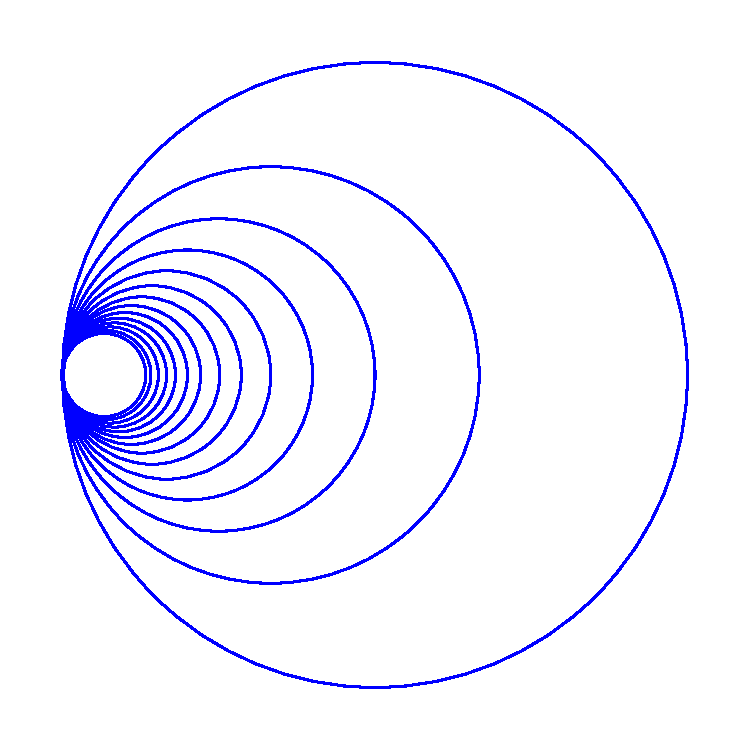
\includegraphics[height=100px]{../figures/hawaiian_earring.pdf}
    \caption{The earring}
\end{figure}

As in the previous example, we look for a family of coverings $q_n:Z_n\longrightarrow X$. In fact, we can take all $Z_n$ to be double covers that are almost trivial --- trivial for all but the $n$-th circle. See Figure \ref{fig:2cover} below.

\begin{figure}[ht!]
    \centering
    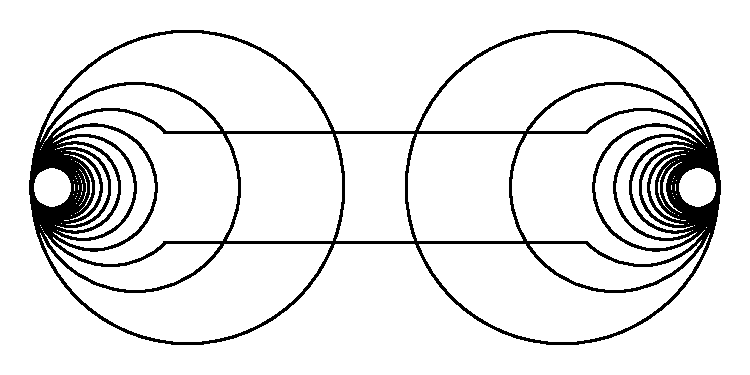
\includegraphics[height=100px]{../figures/hawaiian_earring_2cover.pdf}
    \caption{Example of the double cover $Z_n$, $n=3$}
    \label{fig:2cover}
\end{figure}

% Code for the figure:
% nMax = 15; 
% circles1 = Table[Circle[{1/n, 0}, 1/n], {n, 2, nMax}]; 
% circles1[[3]] = Circle[{1/4, 0}, 1/4, {Pi/4, (7*Pi)/4}]; 
% circles2 = Table[Circle[{2.2 - 1/n, 0}, 1/n], {n, 2, nMax}]; 
% circles2[[3]] = Circle[{2.2 - 1/4, 0}, 1/4, {(5*Pi)/4, (11*Pi)/4}]; 
% d = 1/(4*Sqrt[2]); 
% arc1 = Line[{{1/4, 0} + d*{1, 1}, {2.2 - 1/4, 0} + d*{-1, 1}}]; 
% arc2 = Line[{{1/4, 0} + d*{1, -1}, {2.2 - 1/4, 0} + d*{-1, -1}}]; 
% Graphics[{Black, circles1, circles2, arc1, arc2}, Axes -> False, AspectRatio -> Automatic, 
%   PlotRange -> {{-0.1, 2.3}, {-0.6, 0.6}}, AxesOrigin -> {0, 0}, Frame -> False, 
%   GridLines -> None]

\newpage
Put $Z=\bigsqcup_{n=1}^\infty Z_n$ and $Y=\bigsqcup_{n=1}^\infty X$. The covering map $q$ is given by the disjoint union of all $q_n$, and let $Y$ be the trivial cover of $X$. 

The composition $Z\longrightarrow X$ is obviously not a covering map.

\section*{The End}



\noindent Compiled on \todayymd.

\noindent\home

\end{document}
